% vim: set tw=0 nowrap:
\documentclass[]{soups-poster}
\pdfpagewidth=8.5truein
\pdfpageheight=11truein

\usepackage{booktabs}
\usepackage{pifont}
\newcommand{\xmark}{{\footnotesize\ding{55}}}
\usepackage{lmodern}

\newcommand{\etal}[0]{et~al{.}\@ }
\newcommand{\citep}[1]{\cite{#1}}

\usepackage{listings}
\lstset{%
  basicstyle=\ttfamily\footnotesize,
  keywordstyle=\ttfamily\slshape\footnotesize,
  stringstyle=\ttfamily\bfseries\footnotesize,
  columns=flexible,
  tabsize=2,
  showstringspaces=true,
  %numbers=left,
  numberstyle=\tiny\ttfamily\color{Gray},
  commentstyle=\ttfamily\color{Gray}
}
\newcommand{\code}[2][]{\lstinline[#1]{#2}}
% Autoref line numbers
\providecommand*{\lstnumberautorefname}{line}
% SecPAL
\lstdefinelanguage{apppal}{%
  morekeywords={says,if,where,False,True},%
  otherkeywords={=,0,inf,can-say,can-act-as},%
  morestring=[b]"%
}[keywords,comments,strings]
\lstset{language=apppal}

\usepackage{graphicx}
%\renewcommand{\topfraction}{0.99} % be more aggressive about text around floats
%\renewcommand{\floatpagefraction}{0.99}
\pagestyle{plain}

\usepackage{makecell}% http://ctan.org/pkg/makecell
\renewcommand{\rothead}[2][30]{\rlap{\makebox[4mm][l]{\rotatebox{#1}{\makecell[c]{\footnotesize \textsf{#2}}}}}}%

\begin{document}

\title{Using Authorization Logic to Capture\\User Policies in Mobile Ecosystems}
\numberofauthors{2}
\author{%
  \alignauthor{}
  Joseph Hallett\thanks{With thanks to Igor Muttik at McAfee and N{.}~Asokan at Aalto University for their data and discussions.}\\
  \affaddr{University of Edinburgh}\\
  \email{joseph.hallett@sms.ed.ac.uk}
  \alignauthor{}
  David Aspinall\\
  \affaddr{University of Edinburgh}\\
  \email{david.aspinall@ed.ac.uk}
}
\date\today
\maketitle

\section{Introduction}

Mobile devices let users pick the apps they want to run.
App stores offer a wide range of software for users to choose.
Users pick particular apps for a variety of reasons:
  ordering in the store~\citep{Prata:2012in}, reviews and privacy concerns~\citep{Kelley:2013kc}, and security rules from their employer.

  People fall into patterns when thinking about the privacy issues around apps~\citep{Sadeh:2014vq}.
By capturing these patterns explicitly as policies they can be enforced automatically.
This reduces the burden on users to decide which apps they want.
Security-savvy users may design policies themselves:
  these could be shared with others or used in organisation-wide curated app stores.

We show that we can model security and privacy policies using AppPAL.
Using installation data we explore the extent the policies are being enforced.
We find that only few users appear to be enforcing policies when choosing apps.

% others
% just want help.  By sharing policies users can gain the benefits of expert
%
% written security policies without having to become experts themselves

\section{AppPAL}

We use the AppPAL authorization logic~\citep{Hallett:2014un}, a version of SecPAL~\citep{Becker:2006vh}, to write policies with a precise semantics.
AppPAL describes policies specifiying when an app is installable.
Statements are relative to specific principals, enabling delegation relationships to be expressed.
Delegation is natural in the app store setting: it captures trust relationships among the users, the stores, the developers, and security vendors who vet apps.

Alice, a user, can state that an app is installable:
\begin{lstlisting}
  "alice" says "com.rovio.angrybirds" isInstallable.
\end{lstlisting}
She can specify that an app is only installable if some constraint (checkable by inspecting the app or through static analysis) is true.
She can also delegate parts of the decision to third parties.
They must state specific facts about the app for Alice to accept them.
For example, suppose Alice only wants apps without the \texttt{LOCATION} permission,
and satisfying her \emph{not-malware} requirement.
She trusts McAfee to decide whether the \emph{not-malware} policy is met:
\begin{lstlisting}
  "alice" says App isInstallable
    if "not-malware-policy" isMetBy(App)
    where hasPermission(App, "LOCATION") = False.

  "alice" says "mcafee" can-say
    "not-malware-policy" isMetBy(App).
\end{lstlisting}

Our AppPAL prototype is implemented as a Java library and runs on the
Java and Dalvik virtual machines.

\section{Policies}

In a user study of 725 Android users, Lin~\etal found four patterns that characterise user privacy preferences for apps~\citep{Sadeh:2014vq}.
The \emph{Conservative} users were uncomfortable allowing an app access to any personal data for any reason.
The \emph{Unconcerned} users felt okay allowing access to most data for almost any reason.
The \emph{Advanced} users were comfortable allowing apps access to location data but not if it was for advertising reasons.
Opinions in the largest cluster, \emph{Fencesitters}, varied but were broadly against collection of personal data for advertising purposes.
We wrote AppPAL policies to describe each of these behaviours as increasing sets of permissions:
% The policies are of increasing strictness, each banning more permissions.

\newcommand{\tabtitle}[1]{\textbf{\footnotesize #1}}
\begin{center}
  \begin{tabular}{ r l l l l }
%                                       & \rothead{Conservative} & \rothead{Advanced} & \rothead{Fencesitter} & \rothead{Unconcerned} \\
    \toprule
    \tabtitle{Policy}                  & \tabtitle{C}           & \tabtitle{A}       & \tabtitle{F}          & \tabtitle{U}          \\
    \midrule
    \lstinline{GET_ACCOUNTS}           & \xmark                 & \xmark             & \xmark                & \xmark                \\
    \lstinline{ACCESS_FINE_LOCATION}   & \xmark                 & \xmark             & \xmark                &                       \\
    \lstinline{READ_CONTACT}           & \xmark                 & \xmark             & \xmark                &                       \\
    \lstinline{READ_PHONE_STATE}       & \xmark                 & \xmark             &                       &                       \\
    \lstinline{SEND_SMS}               & \xmark                 & \xmark             &                       &                       \\
    \lstinline{ACCESS_COARSE_LOCATION} & \xmark                 &                    &                       &                       \\
    \bottomrule
  \end{tabular}
\end{center}

%% DA: want to emphasise it is not just about simple sets of permissions.
These simplify the patterns discovered. %~\citep{Sadeh:2014vq}.
But AppPAL constraints
can describe richer policies than permission sets.

% \begin{lstlisting}
% User says "unconcerned-policy" isMetBy(App)
%   if app isAnApp
%   where
%     hasPermission(App, "GET_ACCOUNTS") = False.
%
% User says "fencesitter-policy" isMetBy(App)
%   if "unconcerned-policy" isMetBy(App)
%   where
%     hasPermission(App, "ACCESS_FINE_LOCATION") = False,
%     hasPermission(App, "READ_CONTACT") = False.
%
% User says "advanced-policy" isMetBy(App)
%   if "fencesitter-policy" isMetBy(App)
%   where
%     hasPermission(App, "READ_PHONE_STATE") = False,
%     hasPermission(App, "SEND_SMS") = False,
%
% User says "conservative-policy" isMetBy(App)
%   if "advanced-policy" isMetBy(App)
%   where
%     hasPermission(App, "ACCESS_COARSE_LOCATION") = False.
% \end{lstlisting}

Like other vendors, McAfee classify malware into several categories.
The \emph{malicious} and \emph{trojan} categories describe traditional malware.
Other categories classify PUPs (potentially unwanted programs) such as aggressive adware.
Using AppPAL we can write policies to differentiate between different kinds of malware,
characterising users who allow dangerous apps or those who install merely ``unsavoury'' apps.
\begin{lstlisting}
"user" says "mcafee" can-say
  "malware" isKindOf(App).
"mcafee" says "trojan" can-act-as "malware".
"mcafee" says "pup" can-act-as "malware".
\end{lstlisting}

% We also add two additional policies.
% These policies use the categorization of apps (by the stores) to specify which
% policies based on how we might expect different kinds of apps to behave.
% A user might use app with in-app-purchases in general but decline
% games with them as they can be \emph{Cow Clickers}.
% \begin{lstlisting}
% User says "iap-policy" isMetBy(App)
%   if app isAnApp
%   where
%     hasGooglePlayCategory(App, "GAME") = False.
%
% User says "iap-policy" isMetBy(App)
%   if app isAnApp
%   where
%     hasGooglePlayCategory(App, "GAME") = True,
%     hasPermission(App, "com.android.vending.BILLING") = False.
% \end{lstlisting}

\section{Experiments}

We aim to demonstrate AppPAL as a language for modelling app installation policies.
We want to measure how far users enforce app installation policies informally.
Users have opinions about apps~\citep{Sadeh:2014vq}: but are they acting on them?

\subsection{Methodology}

We want to test how well policies capture user behavior.
Installation data was taken from a partially anonymized\footnote{Users are replaced with incrementing numbers, app names are replaced with hashes to protect sensitive names.} database of installed apps captured by Carat~\citep{Oliner:2013ht}.
By calculating the hash of known package names we see who installed what.
%
The initial database has over 90,000 apps and 55,000 users.
On average each user installed around 90 apps each; 4,300 apps have known names.
Disregarding system apps (such as \texttt{com.android.vending}) and very common apps (Facebook, Dropbox, Whatsapp, and Twitter) we reduced the set to an average of 20 known apps per user.
To see some variations in app type, we considered only the 44,000 users who had more than 20 known apps.
% We removed users for whom we knew less than 20 ; for whom we didn't have a representative sample of installations.
Using this data, and the apps themselves taken from the Google Play Store and Android Observatory~\citep{Barrera:2012iba}, we checked which apps satisfied which policies.

\subsection{Results}

\begin{figure}[!ht]\centering
  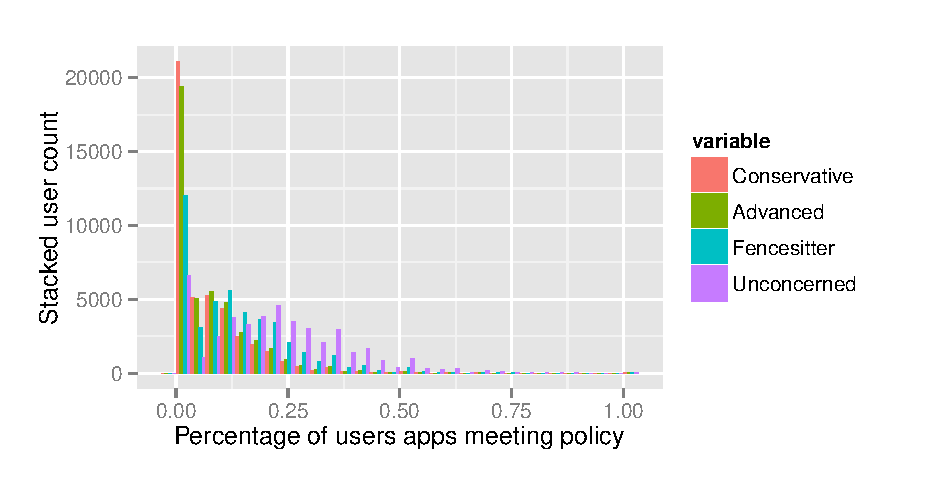
\includegraphics[width=0.90\linewidth]{./tables/lin.eps}
  \caption{Use of policies modelling user behaviour.}
  \label{fig:lin}
\end{figure}

\begin{figure}[!ht]\centering
  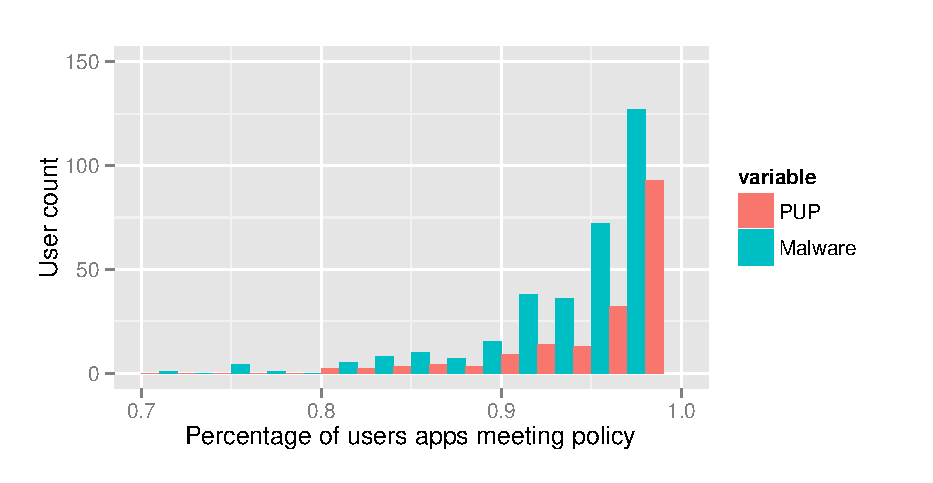
\includegraphics[width=0.85\linewidth]{./tables/malware.eps}
  \caption{Percentage of malware in installed apps for users installing some malicious apps.}
  \label{fig:malware}
\end{figure}

Figure~\ref{fig:lin} shows that the very few users follow these policies,
but a few users who do seem to be installing apps meeting these policies most of the time.
For the unconcerned policy (the most permissive) only 1,606 users (4\%) had 50\% compliance;
  and only 120 users (0.3\%) had 80\% compliance.
For the stricter conservative policy only 60 users were complying half the time, and just 7 more than 80\% of the time.
This suggests that while users may have privacy preferences the majority are not attempting to enforce them.

We found 1\% of the users had a PUP or malicious app installed.
Figure~\ref{fig:malware} shows that infection rates for PUPs and malware is small.
A user is 3 times more likely to have a PUP installed than malware.
Only 9 users had both a PUP and malware installed.
Users who were complying more than half the time with the conservative or advanced policies complied with the malware or PUP policies fully.
This is significant\footnote{P-value: $2.2\times10^{-16}$.} and suggests that users who pick their apps carefully are less likely to experience malware.

\section{Discussion}

Most users seem to use apps irrespective of how uncomfortable they are with the permissions they request.
A small set of users do seem to enforce these policies at least some of the time however.
Exploring where this disconnect comes from is an avenue for future research.
Do users not understand the relationship between apps and permissions~\citep{Felt:2012hma}?
Is enforcing them informally too difficult?

We claim that AppPAL can capture the differences in informal user policies. % AppPAL can filter apps on the basis of these policies.
Using AppPAL we have written short policies describing user behaviour and used these to identify the users following them to varying degrees.
Some limitations of our results include:
\begin{itemize}
\item We do not have the full user purchase history, and we can only find out about apps whose names match those in available databases.  % unmask a subset of installed apps.
  So a user may have apps installed that break the policy without us knowing.
  % This is a   limitation of the Carat data set.
\item Recently downloaded apps used for experiment may not be the same version that users had, in particular, their permissions may differ.
  Permissions tend to increase in apps over time~\citep{Wei:2012id}; so a user may actually be more conservative than our analysis suggests.
  % We might find the apps allowed are more permissive now than when th
  %user installed them. %% SO: what is effect on results?
\end{itemize}

To avoid these limitations, we want to test policies out directly with users, and to explore more complex policies dynamically.
We will do this in two ways.
First, by providing an Android app for AppPAL where a user can check their currently installed apps against predefined (perhaps downloadable) policies.
Second, we want to enable automatically-curated app stores for Android that are parameterised on AppPAL policies.

\bibliographystyle{plain}
\bibliography{abstract}

\end{document}

